\documentclass[11pt]{article}
\usepackage{fullpage}
\usepackage{amsmath, amsfonts}
\usepackage{graphicx}
\DeclareMathOperator*{\argmax}{arg\,max}
\begin{document}
		\section*{Estimating Probabilities from data}
		Suppose you have a dataset $\mathcal{D} = \{\vec{x}_i\}_{i=1}^n \in \mathbb{R}^d$. Each data point $\vec{x}_i$ is drawn independently from $\mathcal{N}(\vec{\mu}, I)$ where $I$ is the $d \times d$ identity matrix.
		\begin{enumerate}
			\item Find the MLE for $\vec{\mu}$.
			\item Assume a standard Gaussian prior on $u$, namely, $P(\vec{\mu}) = \mathcal{N}(0, I)$, find the MAP for $\vec{\mu}$.
			\item Assume the same Gaussian prior on $\vec{\mu}$ in (2), find the posterior distribution $P(\vec{\mu} | \mathcal{D})$. (Hint: the posterior is a Gaussian distribution.)
		\end{enumerate}
		
		\textbf{Solution: }
		
		\begin{enumerate}
		    \item We first find $P(\mathcal{D} | \vec{\mu})$. Since the data is i.i.d., we have 
		    
		    \begin{align*}
		        P(\mathcal{D} | \vec{\mu}) &= \prod_{i=1}^n P(\vec{x}_i | \vec{\mu}) \\ 
		        &= \prod_{i=1}^n \frac{1}{\sqrt{\left ( 2 \pi \right )^d |I|}} \exp \left ( -\frac{\left ( \vec{x}_i - \vec{\mu} \right )^TI^{-1} \left ( \vec{x}_i - \vec{\mu} \right )}{2} \right ) \\
		        &= \prod_{i=1}^n \frac{1}{\left ( 2 \pi \right ) ^{\frac{d}{2}}} \exp \left (-\frac{\left ( \vec{x}_i - \vec{\mu} \right )^T\left ( \vec{x}_i - \vec{\mu} \right )}{2} \right )
		    \end{align*}
		    
		   where we use the fact that $\det I = 1$, and $I^{-1} = I$. 
		   We take the log-likelihood (making the derivative calculation much easier), giving us 
		    
		    \begin{align*}
		        \log P(\mathcal{D} | \vec{\mu}) &= \log \prod_{i=1}^n \frac{1}{\left ( 2 \pi \right ) ^{\frac{d}{2}}} \exp \left (-\frac{\left ( \vec{x}_i - \vec{\mu} \right )^T\left ( \vec{x}_i - \vec{\mu} \right )}{2} \right ) \\ 
		        &= \sum_{i=1}^n \log \left ( \frac{1}{\left ( 2 \pi \right ) ^{\frac{d}{2}}} \exp \left (-\frac{\left ( \vec{x}_i - \vec{\mu} \right )^T\left ( \vec{x}_i - \vec{\mu} \right )}{2} \right ) \right ) \\
		        &= \sum_{i=1}^n \log \left (\frac{1}{\left ( 2 \pi \right ) ^{\frac{d}{2}}} \right ) -\frac{\left ( \vec{x}_i - \vec{\mu} \right )^T\left ( \vec{x}_i - \vec{\mu} \right )}{2} \\
		        &= \sum_{i=1}^n -\frac{d}{2} \log \left ( 2 \pi \right )  -\frac{\left ( \vec{x}_i - \vec{\mu} \right )^T\left ( \vec{x}_i - \vec{\mu} \right )}{2} \\
		        &= -\frac{nd}{2} \log(2\pi) - \sum_{i=1}^n \frac{\left ( \vec{x}_i - \vec{\mu} \right )^T\left ( \vec{x}_i - \vec{\mu} \right )}{2} 
		    \end{align*}
		    
		    We then find the partial derivative with respect to $\vec{\mu}$:
		    
		    \begin{align*}
		        \nabla_{\vec{\mu}} \log P(\mathcal{D} | \vec{\mu}) &= \nabla_{\vec{\mu}} \left ( -\frac{nd}{2} \log(2\pi) - \sum_{i=1}^n \frac{\left ( \vec{x}_i - \vec{\mu} \right )^T\left ( \vec{x}_i - \vec{\mu} \right )}{2} \right ) \\
		        &= \sum_{i=1}^n (\vec{x}_i - \vec{\mu} )
		    \end{align*}
		    
		    To find the derivative of $(\vec{x}_i - \vec{\mu})^T(\vec{x}_i - \vec{\mu})$ we note that $(\vec{x}_i - \vec{\mu})^T(\vec{x}_i - \vec{\mu}) = ||\vec{x}_i - \vec{\mu}||^2_2$, and 
		    $\nabla_x ||x||^2_2 = 2x$, then we can apply the chain rule. Finally, setting the derivative to zero gets us 
		    
		    \begin{align*}
		        &\nabla_{\vec{\mu}} \log P(\mathcal{D} | \vec{\mu}) = 0 \\
		        &\implies \sum_{i=1}^n (\vec{x}_i - \vec{\mu})  = 0 \\
		        &\implies n \vec{\mu} = \sum_{i=1}^n \vec{x}_i \\ 
		        &\implies \boxed{\vec{\mu} = \frac{\sum_{i=1}^n \vec{x}_i}{n}}
		    \end{align*}
		    
		    To verify that this is indeed a maximum, we perform the second derivative test
		    \[\nabla_{\vec{\mu}}^2 \log P(\mathcal{D} | \vec{\mu}) = -nI \]
		    Since the second derivative is the negative definite, we have a local maximum.
		\item To find the MAP, we simply want to find $\argmax_{\vec{\mu}} P(\vec{\mu} | \mathcal{D})$. We know 
		
		\begin{align*}
		    \argmax_{\vec{\mu}} P(\vec{\mu} | \mathcal{D}) &= \argmax_{\vec{\mu}} \log P(\vec{\mu} | \mathcal{D}) \\ 
		    &= \argmax_{\vec{\mu}}  \log \left ( \frac{P(\mathcal{D} | \vec{\mu}) P(\vec{\mu})}{P(\mathcal{D})} \right ) \\
		    &= \argmax_{\vec{\mu}} \log ( P(\mathcal{D} | \vec{\mu}) P(\vec{\mu}) ) \\ 
		    &= \argmax_{\vec{\mu}} \log P(\mathcal{D} | \vec{\mu}) + \log P(\vec{\mu})
		\end{align*}
		
		where we use the monotonicity of the $\log$ function in the first step above. We have already computed $\log P(\mathcal{D} | \vec{\mu})$, leaving
		us only to find $\log P(\vec{\mu})$. We have 
		
		\begin{align*}
		    \log P(\vec{\mu}) &= \log \frac{1}{\sqrt{\left (2 \pi \right )^d |I|}} \exp \left(- \frac{\vec{\mu}^TI^{-1}\vec{\mu}}{2}\right) \\
		    &= -\frac{d}{2} \log 2 \pi - \frac{\vec{\mu}^T\vec{\mu}}{2}
		\end{align*}
		
		Trivially, we have the partial derivative of $\log P(\vec{\mu})$ with respect to $\vec{\mu}$ is $\vec{\mu}$. Thus, 
		
		\begin{align*}
		    &\nabla_{\vec{\mu}} (\log P(\mathcal{D} | \vec{\mu}) + \log P(\vec{\mu})) = 0\\
		    &\implies \sum_{i=1}^n( \vec{x}_i - \vec{\mu}) - \vec{\mu} = 0 \\
		    &\implies (n+1)\vec{\mu} = \sum_{i=1}^n \vec{x}_i \\
		    &\implies \boxed{\vec{\mu} = \frac{\sum_{i=1}^n \vec{x}_i}{n+1}}
		\end{align*}
		
		Again, we test this point by taking the second derivative
		\begin{align*}
            &\nabla_{\vec{\mu}}^2 (\log P(\mathcal{D} | \vec{\mu}) + \log P(\vec{\mu})) = -I(n+1)
		\end{align*}
		
		The second derivative is negative definite so it is a maximum.
		
		\item Intuitively, we can expect the mean to be $\frac{\sum_{i=1}^n \vec{x}_i}{n+1}$ and the variance to be $\frac{1}{n+1}I$, but let us
		see if we can prove it. We have 
		
		\begin{align*}
		    P(\vec{\mu} | \mathcal{D}) &\propto \prod_{i=1}^n \frac{1}{\sqrt{\left ( 2 \pi \right )^d |I|}} \exp \left ( -\frac{\left ( \vec{x}_i - \vec{\mu} \right )^TI^{-1} \left ( \vec{x}_i - \vec{\mu} \right )}{2} \right ) \frac{1}{\sqrt{\left (2 \pi \right )^d |I|}} \exp \left (- \frac{\vec{\mu}^TI^{-1}\vec{\mu}}{2} \right ) \\
		    &= \left ( \frac{1}{\sqrt{(2\pi)^d}} \right )^{n+1} \exp \left (-\frac{(n+1)\vec{\mu}^T\vec{\mu} - 2\vec{\mu}^T\sum_{i=1}^n\vec{x}_i + \sum_{i=1}^n\vec{x}_i^T\vec{x}_i}{2} \right )
		\end{align*}
		
		We know the above has to be a Gaussian distribution. We note that a Gaussian distribution has the form of $c \exp {-\frac{(\vec{\mu}-m)^T\Sigma^{-1}(\vec{\mu}-m)}{2}}$,
		which when expanding the numerator, comes out to be
		
		\[c \exp \left (-\frac{1}{2} \vec{\mu}^T\Sigma^{-1}\vec{\mu} - \vec{\mu}^T \Sigma^{-1} m + \text{const} \right )\]
		
		where $\Sigma^{-1}$ is the inverse covariance matrix.
		
		\pagebreak
		
		We can see that the above is in the same form, and from there we derive that 
		
		\[\Sigma^{-1} = (n+1) I \implies \Sigma = \frac{1}{n+1} I\]
		
		and 
		
		\[\Sigma^{-1}m = \sum_{i=1}^n\vec{x}_i \implies m = \frac{\sum_{i=1}^n\vec{x}_i}{n+1}\]
		
		Thus, 
		
		\[\boxed{P(\vec{\mu} | \mathcal{D}) \sim \mathcal{N} \left (\frac{\sum_{i=1}^n\vec{x}_i}{n+1}, \frac{1}{n+1} I \right )}\]
		    
		\end{enumerate}
	%\section*{Cramer-Rao Inequality (Optional)}
		%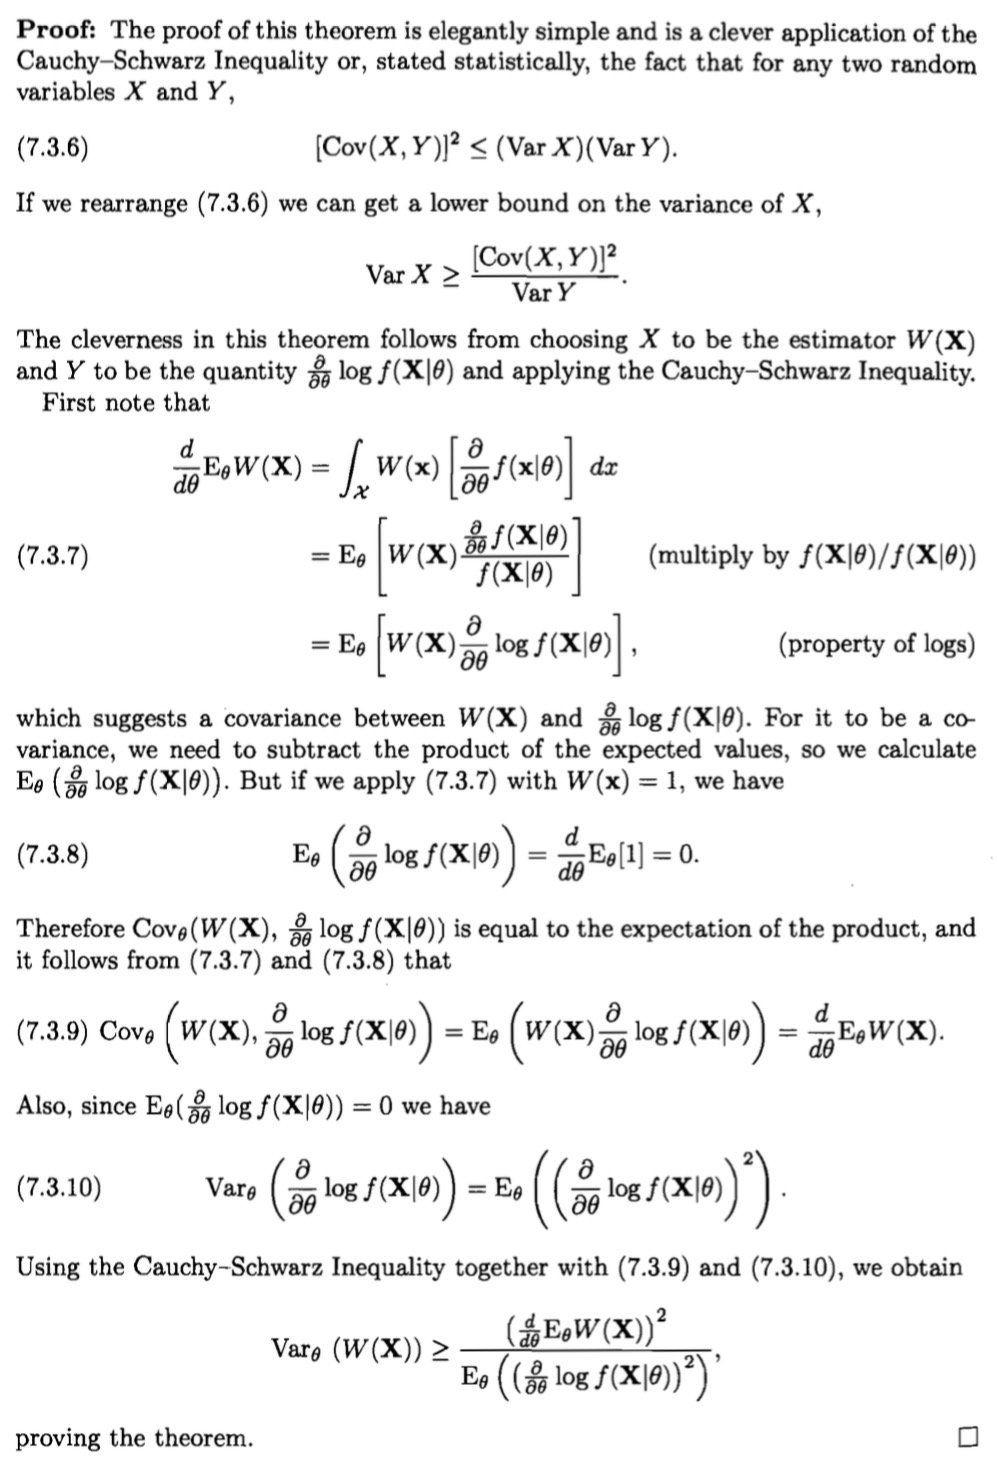
\includegraphics[scale=0.43]{solution_2}\\
		%Note: The proof above is from the book \textit{Statistical Inference} (P335-336) by George Casella and Roger L. Berger.
\end{document}